\chapter{Background}

Thanks to a protective atmosphere, Earth\comment{Oh sure, now you start capitalizing it...} can withstand impacts from dust to boulder-sized objects traveling faster than bullets without so much as a dent on Earth's surface.
While most of these near-Earth objects are extremely small and don't leave much of a trace, the larger objects can leave a light trail\comment{I can guess, but what do you mean by ``light trail'' here?} visible from Earth's surface as they burn up in our atmosphere.
In this chapter, we will discuss the classification of near-Earth objects, the camera system and theory behind our analysis, the current photometry tools we have, along with other existing surveys.\comment{What exactly about other existing surveys?}


\section{Description of Fireballs}

When considering types of near-Earth objects, many names come to mind: asteroids, meteors, meteorites, and fireballs are all often used interchangeably. 
However, there are several key distinctions between these objects.  
Asteroids are the largest of this group and are generally over \SI{10}{\meter} in diameter \cite{steel_meteoroid_1996}. 
These large objects are responsible for large craters that are visibly present on the moon.\comment{Lots of ``large'' in these past two sentences}  
Meteoroids are anywhere between \SI{10}{\micro\meter} and \SI{10}{\meter} and are far more numerious than their asteroid cousins.  

Meteoroids that pass through Earth's atmosphere become meteors.
As meteors pass through the atmosphere, they begin to ablate, or release light.\comment{Ablating and releasing light are not synonymous}
This phenomena happens because the interactions between meteor molecules and air molecules produce lots of energy, some of which goes into the production of light.\comment{Where is the energy coming from? What exactly are these ``interactions''?}
The amount of released light that reaches an observer can be measured in terms of apparent magnitude.
Magnitude is represented on a $\log_10$ scale where dimmer objects are represented by high numbers and brighter objects are lower.\comment{This seems an obvious place for the actual equation and reference.}  
If the meteor releases visible light below an apparent magnitude of $-4$ qualify as bolides, or fireballs.\comment{Sentence is convoluted.}
For reference, Venus is a magnitude $-4.4$ planet while the dimmer Jupiter has a magnitude of $-2.1$ \cite{rao_venus_nodate}.\comment{Venus's magnitude changes as it goes through its phases, so you might want to be specific about which phase you are talking about.}
If an object is massive enough to withstand the pressures of Earth's atmosphere and make it to the surface of Earth, it is classified as a meteorite. 
These are extremely\comment{how much so?} uncommon, but can provide valuable information about the rock's origins.
Figure \ref{jed} summarizes the relationship between these 4 terms.

\begin{figure}[ht!]
  \centering
  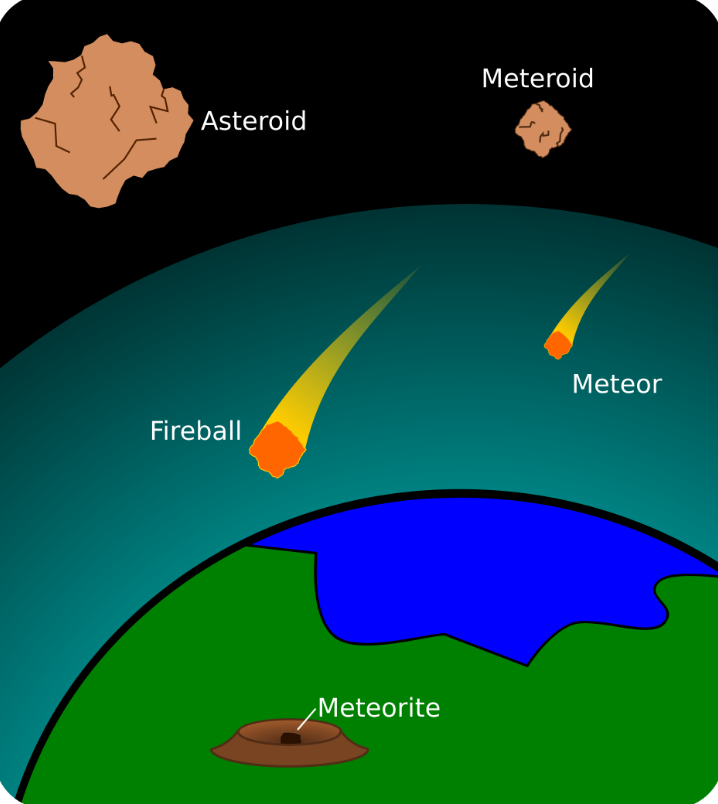
\includegraphics[scale=0.3]{images/jed_zoomedin.png}
  \caption{A depiction of near-Earth object classification.  Asteroids and meteoroids may be found in space, while meteors and their brighter counterpart, fireballs, burn up through Earth's atmosphere.  Unlike ordinary fireballs, meteorites remain intact }
  \label{jed}
\end{figure}

We may further classify near-Earth objects into two categories: sporadic events and meteor shower events.\comment{We aren't really classifying the objects here, rather the fireball events. And the type of event tells us information about the object.}
Meteor showers occur when Earth's orbit crosses paths with the orbit of a collection of debris. 
Such collections often orbit large masses such as Jupiter or the sun \cite{trigo-rodriguez_2006_2007}.  
For example, the Perseid meteor shower has a highly elliptical orbit around the sun as seen in Figure \ref{perceid}.  
A majority of the composition of these showers stems from the decomposition of comets throughout space.\comment{I get it, but that is a heck of a confusing sentence.}

\begin{figure}[ht!]
  \centering
  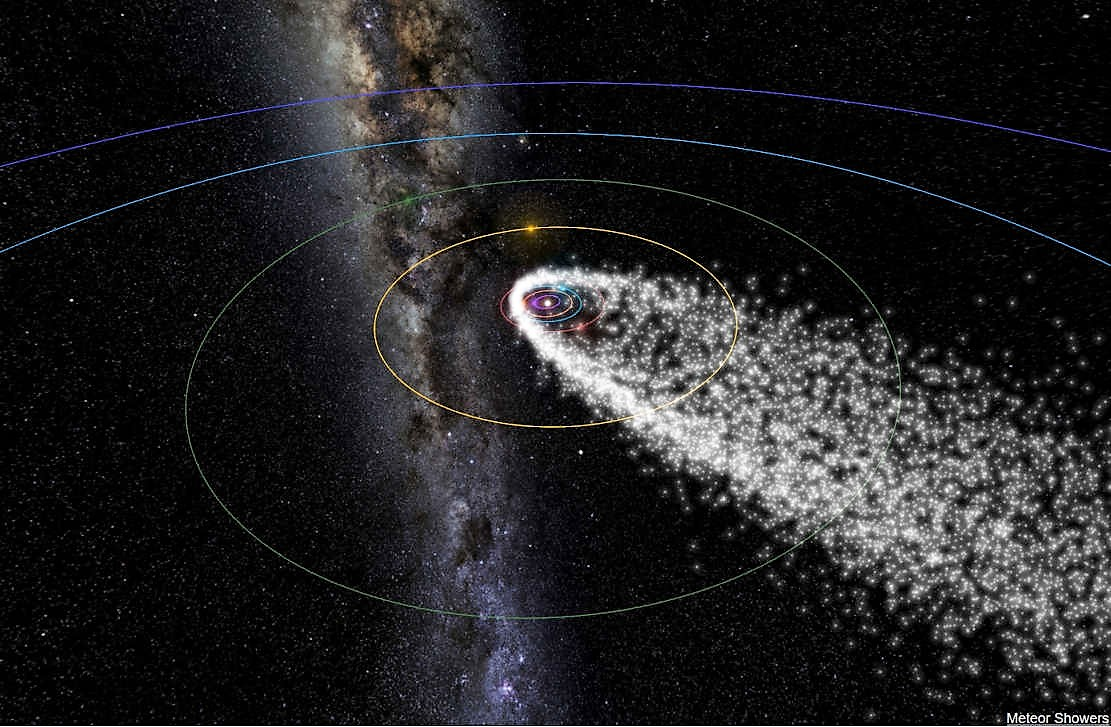
\includegraphics[scale=0.7]{images/persiod_shower.jpg}
  \caption{The Perseid meteor shower and its relation to our solar system.}
  \label{perceid}
\end{figure}

In contrast, there is debris in space that is not connected to any meteor shower. 
These are called sporadic events.\comment{Again, just nomenclature. The event and the object are separate things.} 
Because gravity tends to bring objects together, we see mostly collections of debris.\comment{What are you trying to say here? This is confusing.}
However, when objects escape their collection due to other interactions (gravitational or electromagnetic), they still have a chance of colliding with Earth.\comment{This seems an odd end to the paragraph.}

\comment{I might almost think this whole paragraph could be moved to the Introduction and fit there better.}Studying these near-Earth objects can give us good estimates for how many objects you might expect to see pass through a given area of space within a specific amount of time.
This measurement is called flux.
By determining flux, we can more accurately predict the likelihood of objects in space being hit by near-Earth objects. 
Although the case may have been an extreme one, the space satellite Olympus was struck and destroyed by a meteoroid during the Perseid meteor shower in 1993 \cite{bobrowsky_comet/asteroid_nodate}.
Additionally, given the relationships between the number of objects hitting earth per time for different objects, we can estimate the probability of extremely large impacts on earth.
These estimates, similarly to predictions surrounding volcanic or earthquake activity, give us insight into past events and help us foresee likelihoods of future events.








\section{The D6 AllSky Camera}

The Willamette University D6 Allsky\comment{probably shouldn't be capitalized} camera was created in 2016 to capture images of fireballs streaking through the night sky. 
The aim of the project was to create an economically feasible and highly mobile observational system.
Enclosing a state-of-the-art camera system in a portable structure along with necessary supporting devices, including a controlling Raspberry Pi, Kyle McSwain alongside Dr.\ Jed Rembold were able to get a functioning camera system \cite{mcswain_using_2016}.\comment{This sentence is still really long. I'd break it up more.} 
The assembly resembles a Star Wars astromech droid, and acquired its name from this inspiration.
The enclosure with visible camera is shown in Fig. \ref{droid}.
The D6 allsky camera is currently operational and has been gathering data since the summer of 2018.  
Below, we will discuss the design of the D6 allSky camera while also highlighting what makes it significant.

\begin{figure}[ht!]
  \centering
  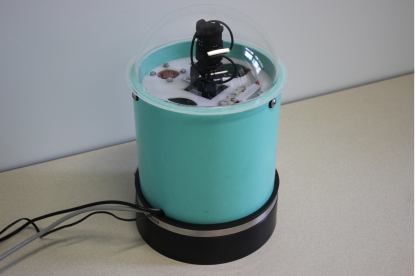
\includegraphics[scale=0.7]{images/allsky_camera.png}
  \caption{The Willamette D6 AllSky Camera (2016) Paired with a little imagination it resembles an astromech droid from Star Wars.\inlinecomment{We should get a new image of this, as it has the sealing cowl along the top now.}}
  \label{droid}
\end{figure}

\subsection{Composition}

The components of the D6 allSky camera are comprised primarily of 5 different pieces: the camera housing, a CCD camera, a thermostat, a digitizer, and the Raspberry Pi to control everything.
The acrylic dome and PVC shell form the exterior of our system. 
The dome itself is a transparent half sphere that sits on top of a PVC cylinder that holds the system together.
It\comment{the dome or the cylinder?} acts as a protective layer between the camera and the outside environment.  
Without this feature, the camera would be subject to rain, snow, dew, bug contamination, and other undesired effects.

The CCD camera is perhaps the most important feature of the camera\comment{too many cameras}.  
The Watec $902$H$2$ CCD camera uses a fish-eye lens to capture incident light from the night's sky.\comment{So the camera is separate from the lens. Probably should talk them separately.}
It was chosen due to its extremely high sensitivity and resolution \cite{mcswain_using_2016}.\comment{Hmmm, it'd be nicer to source some specs here rather than an old thesis.}
While some fireball camera stations are composed of multiple high resolution, more narrow lensed cameras, the D6 AllSky system only contains one camera mostly for economic reasons.\comment{I'd actually flesh this out more in its own paragraph for a nicer comparison to say the CAMS systems.}

Because of its constant use throughout the night, the system itself can get very warm and therefore needs some thermal regulation.
The camera is kept at a relatively constant temperature by a thermostat and a fan system. \comment{Really most of the thermistat is there to \emph{heat} the system to ensure it stays above the dew point.}

The camera outputs an analog signal which requires the use of a digitizer before it can be processed by the Raspberry Pi.
The coaxial signal is sent to the digitizer before connecting to the Raspberry Pi via USB.

\comment{This bit doesn't really seem like it fits in ``Composition"}The Pi then takes the frames from the camera's running video and scans for systematic changes in brightness.
These changes then trigger the recording and storage of a new video, which is saved for further photometric analysis.
By combining these parts into one system, we are able to capture and catalog fireball events.

\subsection{Uniqueness}\comment{Should this be here or after you've talked about other systems? It might actually be better to discuss the background of fireballs and \emph{then} discuss our setup.}

While there are several similarities in the composition of our allSky camera to existing systems, there are several key differences.
The most prominent of these are the size, versatility, and cost of our system.
Around the size of a basketball, the D6 allSky camera is extremely compact.  
Not only is it small, but it only relies on a single power chord for power.  
Because of this, the camera can be easily picked up and relocated to any setting that has a power source.  
The system has low power requirements and it should be possible to run from a battery if remote placement is desirable in the future.
Most other\comment{Very vague. Specific and reference examples would be better.} systems are rooted to extremely powerful computers that have little to no mobility as shown in Fig. \ref{immobile}.

\begin{figure}[ht!]
  \centering
  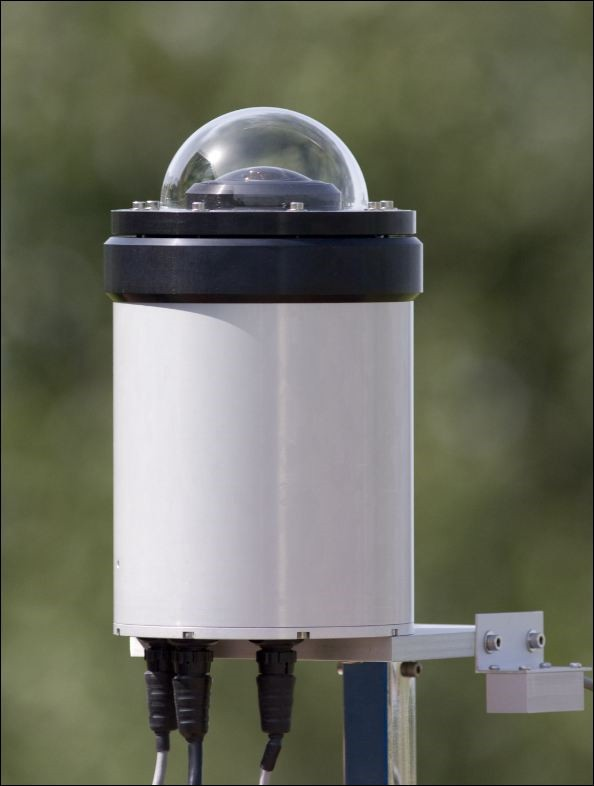
\includegraphics[scale=0.3]{images/othercam.jpg}
  \caption{An entrenched alternative allSky camera.\inlinecomment{Should expand on this. At glance this looks hardly different from ours, and maybe even smaller?}}
  \label{immobile}
\end{figure}

This presents issues related to being rooted in one location.
For example, if a tree were to grow near the camera, it would need to be chopped down or the entire system may need to be relocated.\comment{A tree is a pretty slow growing thing so might not be the best example. What if a new building is erected nearby or a large cooling units is added to the roof of the building?}
With the lightweight and portable D6 allSky camera, relocation is not a difficult process.

Most importantly, the D6 AllSky camera is a less expensive alternative to other fireball analysis tools.\comment{If you are going to say most importantly, you better be able to back that up with hard numbers, which I'm not sure you can.} 
The ingenuity of running initial analysis on a microcomputer allows the D6 allSky camera to cost a fraction of what professional systems cost.
Although large professional organizations produce copious amounts of wonderful data, in the field of fireball research, non-intensified systems outnumber intensified systems $2:1$ \cite{gural_review_2005}. \comment{What the heck does intensified and non-intensified mean in this context?!} 
Providing a cost efficient alternative could be a great way to expand the field of fireball research and in turn provide a better understanding of the near-Earth objects in our solar system.


\section{Photometry}
After collecting videos of potential fireballs, next comes the task of analyzing the videos.
Luke Russell, advised by Dr. Jed Rembold, wrote a photometry program in Python that allows us to get a calibrated light curve for a given video of a fireball.
Simply running a fireball video through his interactive GUI allows us to access information about luminous properties of the fireball.
However, limitations to our photometry must be taken into account.
False positives, extinction, and other error factors must be accounted and corrected for while creating our fireball catalog.

\subsection{Existing photometry tools}
When running a video through the existing photometry script, the user must interact with the program.\comment{Sure?}
After selecting a file to run through the program, the user must find the frame in the video which the fireball first becomes visible.\comment{This process seems spelled out in an overly detailed way here.}
Then, the user must left click on the fireball.
After this, the user must right click on a reference star with a known magnitude.
This step requires a bit of knowledge and will hopefully be automated throughout this project.
After selecting both of these and entering in the known magnitude of the reference star, the program will automatically track the fireball throughout the following frames.
By using Gaussian fits to the photometric data, the program is able to center its view on the fireball and determine its size throughout its path.
Throughout this process, the video also sums the photon counts for each fireball pixel for each frame.
This photon count gives us the magnitude of the fireball at a given point in its path.
Doing this for each frame results in a light curve that shows the magnitude as a function of time.  
By using relations given in the Analysis section\comment{If you are going to talk about them here, you can and should at least introduce the background behind them.}, we are able to calibrate the magnitude and from that calculate the intensity which yield the valuable light curve.
From this light curve, we can then move on to further analysis.

\subsection{Planes, \st{Trains} Bugs, and \st{Automobiles} Extinction}

\begin{figure}[ht!]
  \centering
  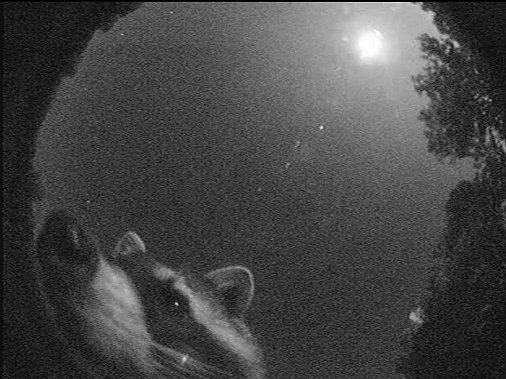
\includegraphics[scale=0.3]{images/racoon_cam.jpg}
  \caption{An elusive fireball/raccoon hybrid.}
  \label{raccoon}
\end{figure}

While it is able to capture fireballs, the D6 allSky camera still picks up a great deal of false positives.
In an initial sample of over $700$ videos, only $2$ of them contained real events.
The vast majority of the videos were of bugs crawling across the acrylic dome.
Because the bugs are illuminated by nearby light, they appear to be bright spots traveling across the screen and thus the detection script mistakenly flags them as fireball events.
Moreover, many bugs are featured in several videos as they have a tendency to move, stop somewhere, and move again.
While this is somewhat problematic, we aim to implement several steps to limit the number of false positive bug cases.\comment{Should have talked about what those would be, but definitely should now!}

In addition to bugs, other events such as airplanes, satellites, and Iridium flares provide false-positive videos.
Their near-linear motion and bright presence are an instant trigger for the fireball detection.
This is a more difficult bug to fix when compared to the bug bug :).
These two cases are just small examples of false positives that result in difficult data to process.\comment{What two cases? The end of this paragraph is a bit disjointed}

\begin{figure}[ht!]
  \centering
  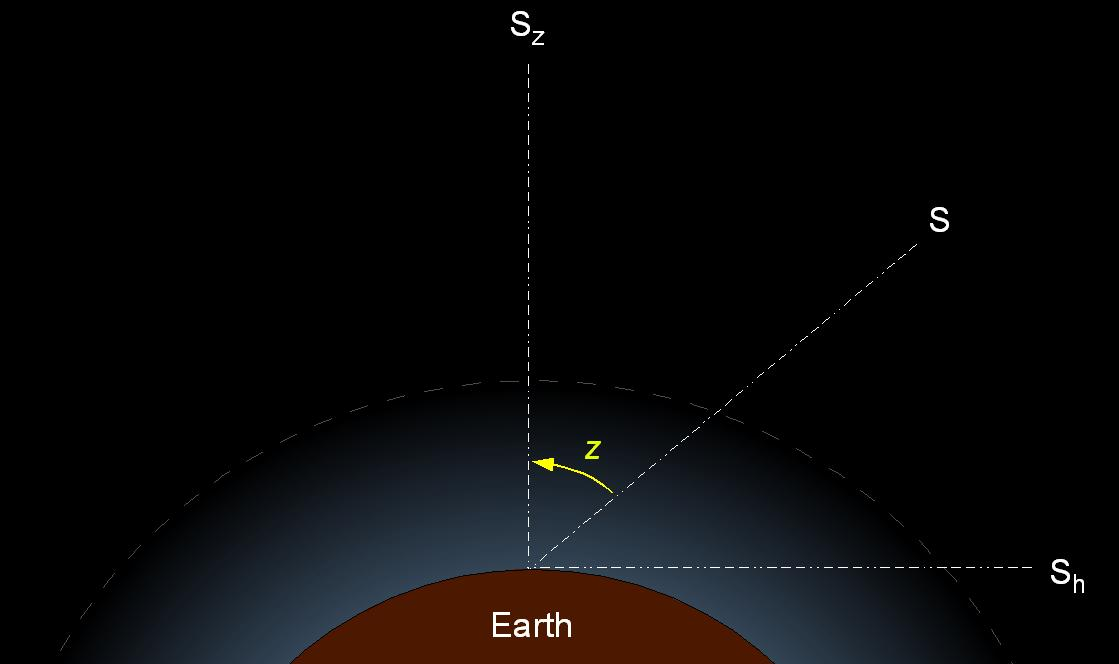
\includegraphics[scale=0.4]{images/extinction.JPG}
  \caption{A depiction of atmospheric extinction.\inlinecomment{This isn't really a depiction so much as a very rough diagram showing some direction. A depiction would be clear evidence of an object of constant brightness seeming dimmer near the horizon.}}
  \label{extinc}
\end{figure}

A larger problem in data analysis stems from the phenomena of atmospheric extinction.
As shown in Figure \ref{extinc}\comment{references to an image should always come before the image}, we observe that when looking close to the horizon (S$_h$ in the image), light must travel through a larger volume of atmosphere than it does for an observation close to the zenith (S$_z$ in the image).  
Because the light travels through more atmosphere, more of the light is absorbed by gases or scattered by air particulates \cite{noauthor_atmospheric_nodate}.\comment{Can we not find a better reference for this?}
A prime example of atmospheric extinction is that of the Sun. 
When directly overhead, the Sun is at its brightest and one should never directly look into it.
However, close to the horizon, the Sun appears more red and can be looked at directly.
Because a rising or setting Sun's rays must travel through more atmosphere, they are scattered due to this extinction and become more comfortably visible.
Part of this project will include accounting for atmospheric extinction in a secondary photometric analysis script.\comment{What does this involve?}

\section{Analysis\inlinecomment{Should come up with a different name for this}}

When creating the catalog, we must first recognize real events.\comment{What exactly does this mean? Or why is it the lead-off sentence of this section?} 
After running the videos of those events through our photometry script, further efforts must be made to calculate properties such as luminous efficiency, total calibrated energy, velocity, and mass.




\subsection{Parameters of Interest}

When analyzing our fireball sample, we will make several key assumptions.  
Firstly, we assume the velocity of the fireball to be traveling at \rule{1cm}{.1pt} meters per second.\comment{This is variable and can be estimated from the type of shower or sporadic that the event corresponds to}
Additionally, we will assume a luminous efficiency of \rule{1cm}{.1pt}.\comment{This we actually need to find a source for. We should both look into that.}

Equation \ref{eq:mass} can be used to determine the initial mass of an ablating meteor,
\begin{equation}
m = \int \frac{2L}{\tau v^2} dt
\label{eq:mass}
\end{equation}
where $L$ is the luminosity, $dt$ is the change in time, $v$ is velocity, and $tau$ is the luminous efficiency. \comment{How are you supposed to know the luminosity?}
This will give us an estimate for the initial mass of the object in question.
Paired with our assumption that fireballs on average have a density\comment{this is an easier source to find. Can check my disseration if struggling to find a source.} of \rule{1cm}{.1pt} and a generally spherical shape, we can calculate the diameter using Equation~\ref{eq:diameter}.
\begin{equation}
d = 2(\frac{3m}{4\pi \rho})^{1/3}
\label{eq:diameter}
\end{equation}
Here $\rho$ represents the density of the fireball prior to entering the atmosphere.\comment{Is the density changing appreciably throughout?}

In addition to calculating the mass and diameter of the fireball, we also aim to calculate the optical energy and total calibrated energy.
These can be calculated using equations.

Insert energy equations here.  I do not know where they exist.\comment{This seems very backwards to me. You have to know the optical energy already, that is what you gathered in the form of the light curve in a calibrated form. I'm actually more concerned about finding the luminosity at the moment given that we aren't going to have an accurate gauge of the distance to the fireball. I guess we are going to have to estimate it from height in the atmosphere, but this will bear examination.}

\subsection{Flux}

The most important data yield we hope to get is a flux consistent with that of other existing surveys.\comment{Terminology here. We really want to get a mass distribution consistant with other surveys. That is the more exact measurement. The flux probably agrees if that does. If the mass distribution doesn't agree but the flux does, then that probably tells us something more about our calibration than our system.}
We hope to collect data that matches the following equation:\comment{100\% this should be presented in light of what others have found and that we'd like to check our results against. You don't really gather data to see if it matches an equation.}
\begin{equation}
\log N = a_0 - b_0\log E
\label{eq:browneq}
\end{equation}
where $N$ is the total number of objects colliding with earth each year and $E$ is the respective energy of the sample in kilotons \cite{brown_p_flux_2002}.
In this equation, $a_0 = 0.5677 \pm 0.015$ while $b_0 = 0.90 \pm 0.03$.\comment{You need to make absolutely clear that this is an empirically derived equation. There is no theory here.}
This relationship is known as a power law, and many professional allSky systems' data match it well.\comment{This sentence seems pointless when you can just show them the image indicating as much. In fact you should really lead with the image.}
The flux is dependent on three things: the number of events, the time of observation, and the area of the sky observed.\comment{THIS is what you should be leading with}
The longer we use the system, the more precise, but not necessarily more consistent, our flux will be.\comment{I get what you are saying, but this seems a bit disjointed and then you don't follow up or discuss any more about it.} 

One factor that is particularly difficult to deal with when considering flux is the area of the sky that is being observed at a given time.
Using basic trigonometry, we can work out that:
\begin{equation}
\text{Sky Coverage} = \Omega(h+r)^2
\label{eq:skycov}
\end{equation}
where $\Omega$ is the steradian, or solid angle from earth, $h$ is the height above Earth's surface, and $r$ is the radius of Earth. \comment{All important equations should have a number and be referenced by that number in the text. If an equation isn't important enough to be referenced directly in the text, it shouldn't get a number.}
The CCD fish-eye camera that we use spans approximately $140\deg$.
Assuming that the height of the fireball is approximately $75$km from Earth's surface, we learn that our camera covers about $119,000$km$^2$ of sky.
That area translates to about $0.023$ percent of Earth's total surface.\comment{Is this comparing sky area to Earth area? Seems a little odd.}
This fact solidifies the importance of many fireball camera systems, as an individual only covers a small fraction of Earth's total surface area.

One might naively assume that the total observation area would remain consistent each night.
However, one must consider clouds and fog when calculating the overall sky area covered.
This consideration will be dealt with in our secondary analysis and is further discussed in the methods section.


\section{Existing Surveys}
While amateur astronomers and low-budget systems capture useful information, larger professional systems act as a vitally important comparison point.
Because many professional surveys are composed of multiple cameras working in unison, they have the advantage of multiple perspectives on a singular event.
This leads to more precise measurements of parameters like velocity, apparent magnitude, and location.
Individual events captured by an individual observer do contribute to the pursuit of knowledge.
However, a small camera system that cannot yield similar data to more professional surveys serves only a marginal amount of utility.


Cameras for AllSky Meteor Surveillance (CAMS), the SPanish Meteor Network (SPMN), and the Lincoln Near Earth Asteroid Research (LINEAR) program are examples of well-established existing meteor observing surveys.\comment{Worth mentioning NASA's Allsky Fireball Network? Or is that folded into one of the others? (CAMS?)} 
All of these programs are continuously acquiring data and adding their findings to existing databases.  
Much of this data is widely available online, but vary from survey to survey.


\subsection{CAMS}
Funded by NASA, Cameras for Allsky Meteor Surveillance (CAMS) aims to verify minor meteor showers and trace them back to their existing parent comets \cite{jenniskens_cams:_2011}.  
The project was created by Peter Jenniskens and is based in California.  
The CAMS network is spread across 3 different locations and consists of over 60 cameras.
Each camera is has a relatively narrow field of view $~30\deg$.\comment{They have way more than this now don't they?}
Although they individually cover a small area, multiple cameras overlapping in field of view contribute to a large sky coverage.\comment{I don't think this is true. You can still only see horizon to horizon from a particular area. They do get a much higher resolution image of the sky though, and less optical warping due to the fisheye effect.} 
CAMS uses powerful CCD cameras to detect extremely dim meteors (up to around $+5$ mag).\comment{I was under the impression they were basically the same camera as ours. Should check or report better numbers as to what they are using.}
By spreading their cameras across three separate locations, the CAMS research group can measure precise trajectories of incoming meteors. 
Similarly to the phenomena of trying to catch a baseball with only one eye open, confidently capturing a three dimensional trajectory of a fireball is extremely difficult when using only one camera.\comment{I get what you are trying to say here but I'd expand on it a bit more. A single camera gets us a position vector but with no concept of depth. Two cameras will result in two position vectors and then we can see where they could cross to figure out the depth.}
Consisting of 3 cameras located within 25 miles of one another, as seen in Figure \ref{trio}, the CAMS survey have a median trajectory error of \ang{0.31}\comment{what does this even mean in terms of a trajectory?} and a median speed error of \SI{0.53}{\kilo\meter\per\second} \cite{jenniskens_cams:_2011}. 

\begin{figure}[ht!]
  \centering
  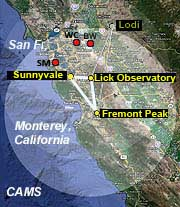
\includegraphics[scale=0.7]{images/CAMS_trio.jpg}
%   \setcaptioncitation{http://cams.seti.org/maps.html}
  \caption{The three CAMS network stations within a 50 mile radius. \inlinecomment{I'd make this image a bit bigger.}}
  \label{trio}
\end{figure}

Accurate trajectories are particularly useful in back-tracing the motion of the meteor's orbit.  
The CAMS team has reduced over $320,000$ of these orbits \cite{noauthor_cameras_nodate}\comment{This should really have a proper paper citation.}. 
In addition to calculating orbits, CAMS also uses their precise velocity measurements to draw relations between speed and other properties. 
Figure~\ref{fancyCAMS} shows the relationship between the apparent incident speed and peak magnitude.\comment{This is actually kinda of interesting, but I'm not sure if it really has a good direct impact on what we are doing or testing. With only a single camera at the moment, we won't have a method of precisely predicting the speed, so we can't really try to replicate this. I suppose we could try with assumed speeds and see how it compares, but if comparing to this is going to be difficult I have to question if is worth showing here.}

\begin{figure}[ht!]
  \centering
  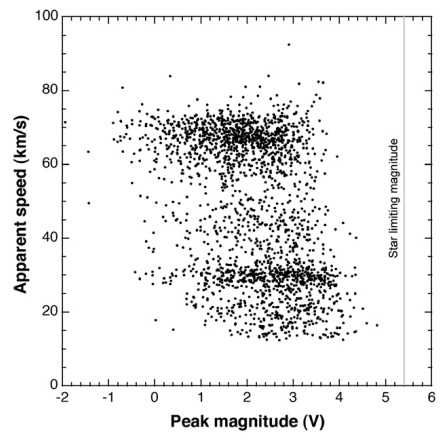
\includegraphics[scale=0.6]{images/CAMS_plot.png}
  \caption{Relationship between incident apparent speed and peak magnitude for CAMS data taken in November of 2010 \cite{jenniskens_cams:_2011}.}
  \label{fancyCAMS}
\end{figure}


Although the plot itself doesn't show a linear relationship, when considering the two subsets of relatively higher and lower incident speeds, we can see a general trend.
That trend shows that lower incident speed meteors tend to have slightly dimmer peak magnitudes. 



\subsection{SPMN}

The SPanish Meteor Network (SPMN) works extremely similarly to the CAMS project.  
It consists of 25 observation stations located across Portugal and Spain \cite{trigo-rodriguez_2006_2007}.\comment{Does SPMN use classic fisheye cameras though?}
Figure~\ref{SPan} shows the approximate coverage of these stations along with some proposed locations (in green), from a satellite point of view.  

\begin{figure}[ht!]
  \centering
  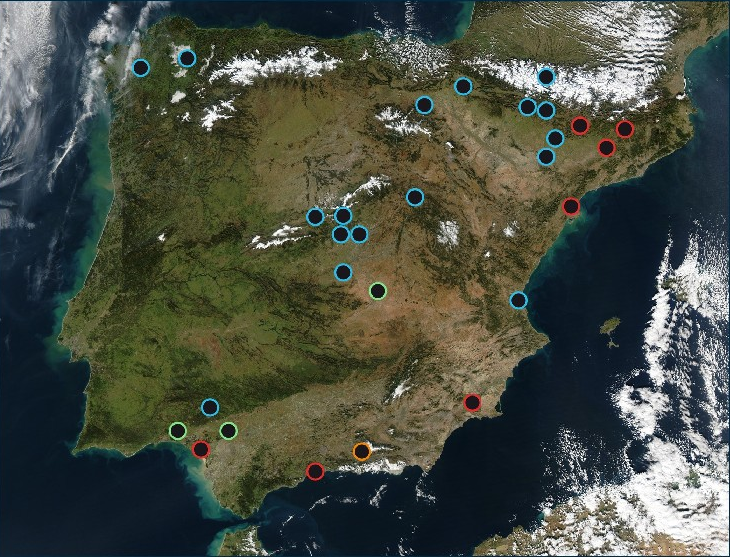
\includegraphics[scale=0.3]{images/satalite_of_love.png}
  \caption{Satellite view of the SPanish Meteor Network's sky coverage across $25$ existing and $3$ proposed observation stations  \cite{noauthor_presentation_nodate}. \inlinecomment{What are the 3 proposed ones? What do all the different colors mean? And this isn't really SKY coverage is it? These are just the camera locations. Their sky coverage would extend over much larger overlapping areas right?}}
  \label{SPan}
\end{figure}

In addition to becoming the first organization in Spain to successfully calculate the orbital path of a meteor, this organization revolutionized fireball research by developing the first CCD allSky cameras \cite{noauthor_presentation_nodate}\comment{Again, this really should have a full paper citation. Look for early papers from Ortiz.}.
These cameras are now in use all across the world.
While the SPMN and CAMS are extremely powerful research organizations, their study of meteors only slightly overlaps with the research being discussed in this paper.\comment{This should be a new paragraph yes?}
Because of their high grade equipment, they are able to capture data from extremely dim sources.
Fireballs, quantified by a magnitude below $-4$, compose only a small fraction of the meteors analyzed by these organizations.
Fortunately, other organizations focus specifically on larger and brighter events.

\subsection{Other research groups}

There are a multitude of ways that one can attain information about a fireball.  
All the aforementioned surveys have employed the use of photometric data.
In contrast, Peter Brown took data from the Department of Defense and the Department of Energy space-based systems in geostationary orbits.
The original purpose of these systems is to detect signatures of explosions near Earth's surface, but the system occasionally picks up false positives in the form of ablating bolides.  
Because the systems detect the amount of power released, Brown and others have used the systems to approximate a fireball's energy.
In a 2002 article published by \textit{Nature}, Brown estimated the optical energies of around 300 bolides.
Drawing from this data set and other existing data sets, Brown created compiled Equation~\ref{powerlaw}, which relates bolide energy to the number of impacts on Earth each year. 

\begin{figure}[ht!]
  \centering
  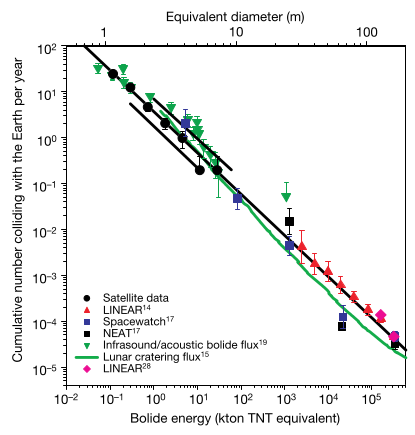
\includegraphics[scale=0.7]{images/flux_brown.png}
  \caption{A plot of bolide flux using an conglomeration of data \cite{brown_p_flux_2002}.}
  \label{powerlaw}
\end{figure}


Figure \ref{powerlaw} shows this relationship alongside data taken from many different research groups.\comment{The figure here should really come before the equation. Brown compiled the figure, when then gave an approximate best fit line equal to the equation.}  
In his research, Brown used existing assumptions (mentioned in the Analysis section) for the blackbody distribution\comment{Wait, what was this?} and the velocity.\comment{Brown issued an update to this within the last 5 years. Do you not have that paper? I thought you did.}

\newpage
\inlinecomment{We talked about much of this yesterday PJ, but I think I'd do some serious rearranging of your background now that you have much of the details down. Something more along the lines of:
	\begin{itemize}
		\item The goal: testing our setup by comparing to Browns compiled energy distribution
		\item What a fireball is
		\item What we need to recreate that plot:
			\begin{itemize}
				\item Event detection
					\begin{itemize}
						\item Description and composition of our camera system
					\end{itemize}
				\item Photometric calibration
					\begin{itemize}
						\item Luke's code
					\end{itemize}
				\item Calibrated magnitude to initial meteor energy/mass
				\item Time observed
				\item Area of sky observed
			\end{itemize}
		\item Current allsky networks (but I might just merge this into event detection actually)
	\end{itemize}
	The benefit of breaking things up into a scaffolding similar to the above is that these are the things you need to figure out to arrive at your conclusion. So they are by necessity also the things that a reader should be familiar with to understand the rest of your project. And focus mainly just on the theoretical underpinnings. You'll explain the experimental/computation steps you did in the methods section. This is just to give the theoretical framework so that your later decisions and choices make sense to the reader. Sometimes its is hard to see what fits where until you actually start writing those later sections though, so if in doubt leave it here for the time being and maybe later you'll end up moving some of it to the methods.
}



